\documentclass[11pt, oneside]{article}   	% use "amsart" instead of "article" for AMSLaTeX format
\usepackage{geometry}                		% See geometry.pdf to learn the layout options. There are lots.
\geometry{letterpaper}                   		% ... or a4paper or a5paper or ... 
%\geometry{landscape}                		% Activate for for rotated page geometry
%\usepackage[parfill]{parskip}    		% Activate to begin paragraphs with an empty line rather than an indent
\usepackage{graphicx}				% Use pdf, png, jpg, or eps� with pdflatex; use eps in DVI mode
								% TeX will automatically convert eps --> pdf in pdflatex		
\usepackage{amssymb}
\usepackage{amsmath}
\usepackage{parskip}
\usepackage{color}

\title{On the sphere}
%\author{The Author}
%\section{}
% \subsection*{R code}
\date{}							% Activate to display a given date or no date

\graphicspath{{/Users/telliott_admin/Dropbox/Tex/png/}}

% \begin{center} 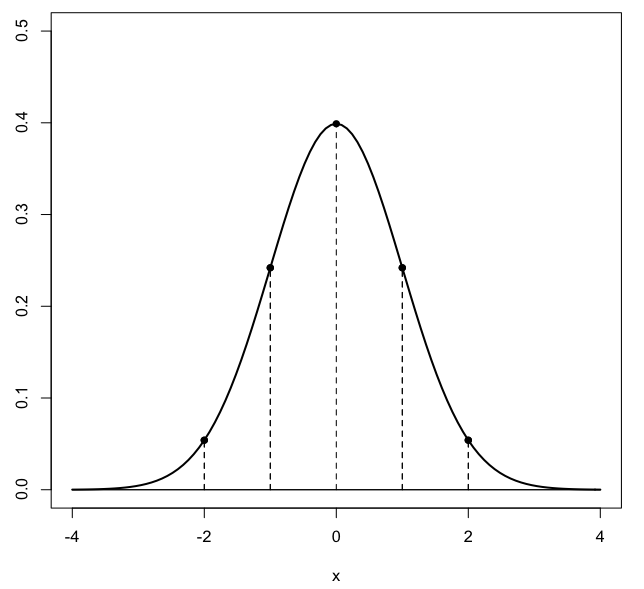
\includegraphics [scale=0.4] {gauss3.png} \end{center}
% \begin{bmatrix} a  &  b \\ c  &  d \end{bmatrix}
% \bigg |_

\begin{document}
\maketitle
\large
%\noindent

To repeat the beginning of the write-up on parametrization of the sphere, we said that:

A sphere centered at the origin is defined as the set of points $x,y,z$ at a distance $\rho$ away from $(0,0,0)$, leading to the equation $x^2 + y^2 + z^2 = \rho^2$.  We are looking for a "parametrization" or relationship between $x,y,z$ coordinates and spherical coordinates in terms of one radial and two angular variables.  These are usually called $\rho, \theta$, and $\phi$.  

If we think of the vector $<x,y,z>$ to a point on the sphere, then $\theta$ is the angle it makes going ccw from the positive $x$-axis and ranges from $0 \le \theta \le 2\pi$.  $\phi$ is the "polar" angle that the same vector makes with the positive $z$-axis and ranges from $0 \le \phi \le \pi$.
\vspace{5 mm}

\noindent
The projection of $\rho$ in the $xy$-plane is $r$.
\[ r = \rho \cos (\frac{\pi}{2} - \phi) = \rho \sin \phi \]
\[ x = r \cos \theta = \rho \sin \phi \cos \theta \]
\[ y = r \sin \theta = \rho \sin \phi \sin \theta \]
\[ z = \rho \sin (\frac{\pi}{2} - \phi) = \rho \cos \phi \]

We went on to analyze the Jacobian and generate this equation for the volume element
\[ \rho^2 \sin \phi \ d \rho \ d \phi \ d \theta \]
and for the volume as a triple integral
\[ \int_{\theta = 0}^{2\pi} \int_{\phi=0}^{\pi} \int_{\rho=0}^a \ \rho^2 \sin \phi \ d \rho \ d \phi \ d \theta \]
Using the figure from \emph{How to ace calculus}
%\begin{center} 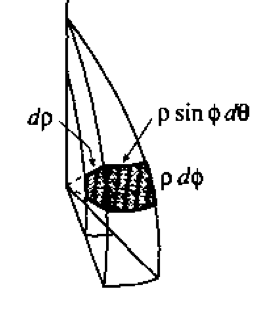
\includegraphics [scale=0.4] {sphere_dV.png} \end{center}
\begin{center} 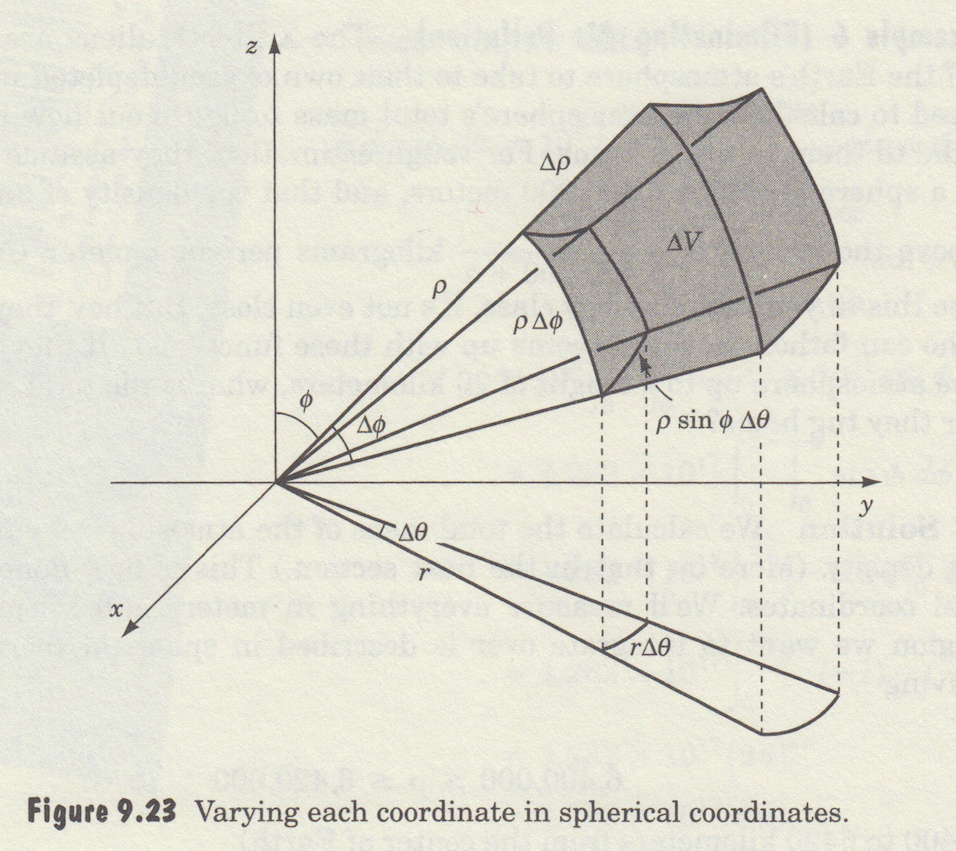
\includegraphics [scale=0.4] {sphcoord.png} \end{center}

We can visualize where these come from.  In particular, the vertical sides of the volume element have length $\rho \ d \phi$, while the horizontal sides are $\rho \ \sin \phi \ d \theta$.  A good way to think about this is that the vertical slices include the vertical axis of the sphere and are "great circles" of radius $\rho$, while the horizontal slices are smaller.  In fact, if we look at the projection onto the $xy$-plane, we have a circle of radius $r$, where $r=x^2 + y^2$, but also $r = \rho \ \sin \phi$.

We can also parametrize the sphere with cylindrical coordinates ($r$, $\theta$, and $z$).  In setting up an integral for the triple volume, we will do $z$ first.  The bounds on $z$ are crucial.  If the radius of the sphere is $R$, then
\[ R^2 = x^2 + y^2 + z^2 \]
but since $r^2 = x^2 + y^2$
\[ R^2 = z^2 + r^2 \]
so $z=-\sqrt{R^2 - r^2} \rightarrow \sqrt{R^2 - r^2}$ and
and for the volume as a triple integral
\[ \int_{\theta = 0}^{2 \pi} \int_{r=0}^{R} \int_{z=-\sqrt{R^2 - r^2}}^{z=\sqrt{R^2 - r^2}} \ dz \ r \ dr \ d \theta \]
The inner integral is just
\[ 2 \sqrt{R^2 - r^2} \]
The middle integral is
\[  \int_{r=0}^{R} 2 \sqrt{R^2 - r^2} \ r \ dr \]
\[ = -\frac{2}{3} (R^2 - r^2)^{3/2} \ \bigg |_{r=0}^R \]
\[ = \frac{2}{3} R^3 \]
We pick up a factor of $2\pi$ from the outer integral, giving the familiar answer.

Cylindrical coordinates gives a nice approach to the problems of the spherical cap and the "cored" apple.

For the spherical cap, we change the lower bound of integration for $z$ to $R-h$ ($h$ being the height of the cap)

\[ \int_{\theta = 0}^{2 \pi} \int_{r=0}^{R} \int_{z=R-h}^{z=\sqrt{R^2 - r^2}} \ dz \ r \ dr \ d \theta \]
The inner integral is
\[ \sqrt{R^2 - r^2} - (R - h) \]
The middle integral is 
\[ \int_{r=0}^{R}(\sqrt{R^2 - r^2} - (R - h)) \ r \ dr  \]
\[ = -\frac{1}{3} (R^2 - r^2)^{3/2} - \frac{1}{2}(R - h)r^2 \ \bigg |_{r=0}^R \]
\[ = \frac{1}{3}R^3 - \frac{1}{2}(R-h)R^2 \]
The final answer is multiplied by $2\pi$.
For the latter problem, we simply change the lower bound of integration for $r$ to $r=a$.

The middle integral is
\[  \int_{r=a}^{R} 2 \sqrt{R^2 - r^2} \ r \ dr \]
\[ = -\frac{2}{3} (R^2 - r^2)^{3/2} \ \bigg |_{r=a}^R \]
\[ = \frac{2}{3} (R^2 - a^2)^{3/2}  \]
And the final answer is 
\[ \frac{4}{3} \pi  (R^2 - a^2)^{3/2}  \]

\end{document}  